\section{Position Based Dynamics} \label{ch2:pbd} %название по-русски
	Рассмотрим принцип работы алгоритма Position Based Dynamics \cite{pbd}, так как данный алгоритм является оснополагающим для последующих алгоритмов симуляции тканей. 
	
	В рамках математической модели, любое симулируемое тело представляет собой набор из $N$ частиц, соединенних $M$ ограничениями. При этом \textbf{состояние частицы $P_i$ в момент времени $t$} задается как:
	\begin{enumerate}[1.]
		\item Положения частицы $p_i(t)$
		\item Обратной массы $1/m_i = im_i$
	\end{enumerate}
	
	Стоит отметить, две важные особенности. Во-первых - размер частицы считается пренебрежимо мал, по отношению к размеру всего тела. Во-вторых - для описания состояния частицы не используется скорость и ускорение данной частицы (в отличие от методов симуляции используемых для обработки физического взаимодействия абсолютно твердых тел).
	
	Под \textbf{ограничением $j$} понимается набор из:
	\begin{enumerate}[1.]
		\item Размерности ограничения $n_j$
		\item Функции $C_j: \mathbb{R}^{n_j}->\mathbb{R}$
		\item Набор индексов частиц, к которым применяется данное ограничение $\{i_1, i_2, ..., i_{n_j}\}, i_k \in [1, ..., N]$
		\item Параметр жесткости $k_j \in [0...1]$
		\item Тип \say{равенства} или \say{неравенства}
	\end{enumerate}
	
	Будем считать, что ограничение $j$ типа \say{равенства} выполнено, когда:
	\begin{equation} \label{eq:constraint-eq}
		C_j(p_{i_1}, p_{i_2}, ..., p_{i_k}) = 0
	\end{equation} 
	
	Если же ограничение $j$ имеет тип \say{неравенства}, тогда будем считать что оно выполнено когда
	\begin{equation} \label{eq:constraint-neq}
		C_j(p_{i_1}, p_{i_2}, ..., p_{i_k}) \ge 0
	\end{equation} 
	
	Как пример, можно привести ограничение \say{пружина}, использующееся для симуляции ткани. Функция $C_j$ такого ограничения будет выглядеть следующим образом
	\begin{equation} \label{eq:constraint-spring}
		C_j(p_{i_1}, p_{i_2}) = |p_{i_1} - p_{i_2}| - d
	\end{equation} 
	где под переменной $d$ понимается длина \say{пружины} в состоянии покоя. В дальнейшей работе будут рассматриваться только ограничения вида равенства, однако ограничение типа неравенства может быть приведено к ограничению типа равенства при помощи построения $C^{'}_{j} = max(0, C_j)$.
	
	Тогда, если заданы частиц и их ограничения, алгоритм PBD будет представляться следующим (\firef{alg:PositionBasedDynamics}) образом.
	
	\begin{algorithm} %[h]
		\SetKwFunction{algoPBDPseudocode}{} 
		\SetKwProg{myalg}{Algorithm}{}{} %write in 2nd agrument <<Algorithm>>, <<Procedure>> etc
		\nonl\myalg{\algoPBDPseudocode}{
			\KwInput{
				время шага симуляции $\delta t$,
				количество итераций $solverIteration$,
				текущее состояние частиц,
				предыдущее состояние частиц,
				ограничения,
				функция суммы внешних сил от положения $f_{ext}(p)$,
			}
			\KwOutput{положение частиц спустя заданное время $p_i(t + \delta t)$}
			
			\For {$\forall p_i $\label{step:pbd-solver-integrate}}{
				$v_i \leftarrow \frac{p_i(t) - p_i(t -\delta t)}{\delta t} + \delta t * im_i * f_{ext}(p_i)$;
				
				$p^*_i \leftarrow p_i(t) + v_i * \delta t $\;
			}
			
			\For{solverIteration \textbf{times}  \label{step:pbd-solver-loop}}{
				$p^*_1, ..., p^*_N \leftarrow projectConstraints(C_1, ..., C_M, n_1, ..., n_M, k_1, ..., k_M, p^*_1, ..., p^*_N, im_1, ..., im_N)$;
			}
			
			\For {$\forall p_i $\label{step:pbd-solver-save}}{
				$p_i(t + \delta t) \leftarrow p^*_i$\;
			}
		}
		\caption{Псевдокод алгоритма Position Based Dynamics}\label{alg:PositionBasedDynamics}
	\end{algorithm}
	\FloatBarrier
	
	Как можно заметить, начинается данный алгоритм является итеративным алгоритмом, выдающим по текущему состоянию тела и прошедшему времени - новое состояние тела. Начинается алгоритм с предсказания новых положений путем численного интегрирования уравнения перемещения частицы методом Стёрмера-Верле\cite{verlet1967computer} (строка \ref{step:pbd-solver-integrate}). Данный метод был выбран неслучайно, т.к. он требует только одного предыдущего значения, а также является более устойчивым чем метод Эйлера. Далее (строка \ref{step:pbd-solver-loop}), $solverIteration$ раз запускается алгоритм $projectConstraints$, задача которого модифицировать предсказанные положения частиц таким образом, чтобы выполнялись  поставленные ограничения. Затем (строка \ref{step:pbd-solver-save}), предсказанные позиции записываются как положения частиц, на момент времени $\delta t$.
	
	Перед тем, как разобраться в принципе работы алгоритма  $projectConstraints$, необходимо найти способ решать задачу для одного ограничения. Для этого возьмем произвольное ограничение и обозначим функцию этого ограничения как $C$. Поставим задачу найти $\delta p^*$ такой что.
	\begin{equation}
		C(p^* + \delta p^*) = 0
	\end{equation}
	Сделать это несложно, достаточно разложить данное равенство в ряд Тейлора
	\begin{equation}
		C(p^* + \delta p^*) \approx C(p^*) + \delta p^* * \nabla_{p^*} C(p^*) = 0
	\end{equation}
	\begin{equation} \label{eq:delta_p_pbd}
		\delta p^* = -\frac{C(p^*)}{|\nabla C(p^*)|^2} * \nabla C(p^*)
	\end{equation}
	
	Таким образом, используя выражение \ref{eq:delta_p_pbd} мы для каждой затронутой частицы можем найти смещение необходимое для удовлетворения данного ограничения, но только в случае если массы частиц равны между собой. Иначе требуется воспользоваться \ref{eq:delta_p_pbd_2}
	
	\begin{equation} \label{eq:delta_p_pbd_2}
		\delta p^*_i = - \frac{im_i}{\sum_l im_l} \frac{C(p^*)}{|\nabla C(p^*)|^2} * \nabla_{p^*_i} C(p^*)
	\end{equation}

	Стоит отметить, что при значении $im_i = 0$ (соответствующее бесконечной массе) не только $\delta p^*_i = 0$, но и внешние силы при интеграции методом Стёрмера-Верле (\firef{alg:PositionBasedDynamics}) не будут влиять на положение вершины. Это означает что таким образом можно \say{закреплять} такие вершины в пространстве, или \say{прикреплять} к другим симулируемым физическим телам.
	
	\begin{algorithm} %[h]
		\SetKwFunction{solveConstraint}{} 
		\SetKwProg{myalg}{Algorithm}{}{}
		\nonl\myalg{solveConstraint}{
			\KwInput{
				размерность ограничения $n$,
				функция ограничения $C$, 
				предсказанные положения частиц $p^*_i$,
				обратные массы частиц $im_i$,
			}
			\KwOutput{необходимый сдвиг для удолветворения ограничению $\delta p^*_i$}
						
			$scaleFactor = {C(p^*_1, ...)} / {\sum_{i}(im_i *|\nabla_{p^*_i} C(p^*_1, ..., p^*_{n})|^2)}$
			
			\For {$\forall p^*_i$}{
				$\delta p^*_i \leftarrow -scaleFactor * im_i * \nabla_{p^*_i} C(p^*_1, ..., p^*_{n})$;
			}
		}
		\caption{Псевдокод алгоритма solveConstraint}\label{alg:SolveConstraint}
	\end{algorithm}
	\FloatBarrier
	
	Для того, чтобы решить задачу для набора ограничений, авторами было предложено 2 алгоритма. 
	
	Первый (\firef{alg:projectConstraintsJacobi}) по словам авторов основан на методе Якоби для решения СЛАУ, хотя функции ограничений не обязаны быть линейными. Идея данного алгоритма заключается в том, чтобы для каждого ограничения вычислить сдвиги соответствующих вершин и сохранить их во временную переменную. Затем, пройтись по всем частицам и применить суммарный сдвиг, домноженный на некий коэффициент.
	
	\begin{algorithm} %[h]
		\SetKwFunction{projectConstraintsJacobi}{} 
		\SetKwProg{myalg}{Algorithm}{}{} %write in 2nd agrument <<Algorithm>>, <<Procedure>> etc
		\nonl\myalg{projectConstraintsJacobi}{
			\KwInput{
				шаг $\alpha$,
				ограничения,
				предсказанные положения частиц $p^*_i$
			}
			\KwOutput{новые положения частиц $p^*_i$}
			
			\For {$\forall C_j $}{
				$tmp \leftarrow solveConstraint(n_j, C_j, p^*_{i_{1}}, ..., p^*_{i_{n_j}}, im_{i_{1}}, ..., im_{i_{n_j}})$;
				
				\For {$\forall tmp_l $} {
					$offsets_{i_l} \leftarrow offsets_{i_l} + k_j * tmp_{l}$;
				}
			}
			
			\For {$\forall p^*_i $}{
				$p^*_i \leftarrow p^*_i + \alpha * offsets_i$;
			}
		}
		\caption{Псевдокод алгоритма projectConstraints использующего метод Якоби}\label{alg:projectConstraintsJacobi}
	\end{algorithm}
	\FloatBarrier

	Второй (\firef{alg:projectConstraintsGauss}) по словам авторов основан на методе Гаусса-Зейделя для решения СЛАУ. Данный метод отличается от предыдущего тем, что сдвиги применяются на частицы сразу, а не накапливаются.


	\begin{algorithm} %[h]
	\SetKwFunction{projectConstraintsGauss}{} 
	\SetKwProg{myalg}{Algorithm}{}{} %write in 2nd agrument <<Algorithm>>, <<Procedure>> etc
	\nonl\myalg{projectConstraintsGauss}{
		\KwInput{
			ограничения,
			предсказанные положения частиц $p^*_i$
		}
		\KwOutput{новые положения частиц $p^*_i$}
		
		\For {$\forall C_j $}{
			$tmp \leftarrow solveConstraint(n_j, C_j, p^*_{i_{1}}, ..., p^*_{i_{n_j}}, im_{i_{1}}, ..., im_{i_{n_j}})$;
			
			\For {$\forall tmp_l $} {
				$p^*_i \leftarrow p^*_i + k_j * tmp_{l}$;
			}
		}
		
	}
	\caption{Псевдокод алгоритма projectConstraints использующего метод Гаусса-Зейделя}\label{alg:projectConstraintsGauss}
	\end{algorithm}
	\FloatBarrier
	
	Как можно заметить, оба алгоритма ориентируются на итеративные алгоритмы решения СЛАУ. Для выбора между этими двумя алгоритмами, авторы оригинальной статьи поставили мысленный эксперимент (\firef{fig:jacobi_vs_gauss}):
	
	\begin{enumerate}[1.]
		\item рассматривается 3 частицы $p_1, p_2, p_3$. Частицы $p_1, p_3$ закреплены
		\item рассматривается 2 ограничения \say{пружина}: $C_1(p_1, p_2)$ с длиной покоя $l_1$ и $C_2(p_2, p_3)$ с длиной покоя $l_2$
		\item исходя из приведенного на рисунке положения частиц видно, что оптимальным положение частицы $p2$ является точка пересечения представленных дуг, имеющих радиусы $l_1$ и $l_2$
		\item проводится одна итерация алгоритмом основанным на методе Якоби и одна итерация алгоритмом основанным на методе Гаусса-Зейделя
		\item В результате поставленного эксперимента, первый алгоритм сходится медленнее чем второй.
	\end{enumerate}
		
	\begin{figure}[h!] 
		\center
		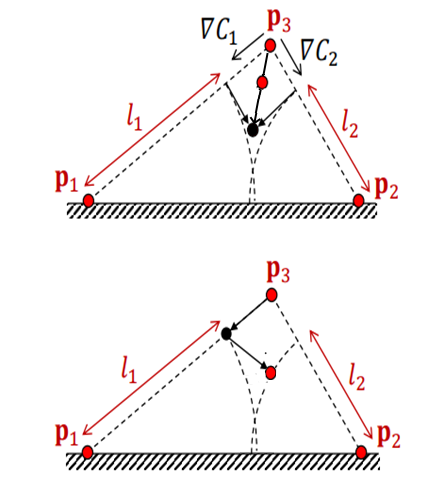
\includegraphics [scale=0.5] {my_folder/images//jacobi_vs_gauss}
		\caption{Эксперимент поставленный авторами статьи.\newline Сверху итерация алгоритмом основанным на методе Якоби, снизу итерация алгоритмом основанным на методе Гаусса-Зейделя}
		\label{fig:jacobi_vs_gauss}  
	\end{figure}
	
	Помимо мысленных экпериментов, авторами были поставлены и численные эксперименты с использованием компьютера. По их словам, первый алгоритм всё ещё сходится медленнее, требует дополнительный объем памяти, требует выбора константы $\alpha$, но достаточно просто может быть распараллен. С другой стороны, алгоритм основанный на методе Гаусса-Зейделя сходится быстрее, не требует дополнительного объема памяти, но результат будет зависеть от порядка обхода и в зависимости от выбранного порядка обхода может быть или не быть распараллелен.

%% Вспомогательные команды - Additional commands
%
%\newpage % принудительное начало с новой страницы, использовать только в конце раздела
%\clearpage % осуществляется пакетом <<placeins>> в пределах секций
%\newpage\leavevmode\thispagestyle{empty}\newpage % 100 % начало новой страницы